% !TEX encoding = UTF-8
% !TEX TS-program = pdflatex
% !TEX root = ../tesi.tex

%**************************************************************
\chapter{Progettazione e codifica}
\label{cap:progettazione-codifica}

%**************************************************************
\section{Framework e tecnologie per lo sviluppo}
\label{sec:framework}
\subsection*{Python}
Python è un linguaggio di programmazione pensato per la ricerca. Per questo linguaggio sono stati sviluppati la maggior parte dei framework che trattano l'intelligenza artificiale (come TensorFlow). Questo vale anche per l'algoritmo di clustering presentato nell'introzione\ref{creazione_regole}.\\
Assieme al tutor aziendale, abbiamo scelto questo linguaggio per i seguenti motivi:
\begin{itemize}
    \item permette di soddisfare il requisito di modularità del codice (requisitio RO-6): il codice prodotto è compatibile con quello dell'algoritmo di clustering;
    \item possiede dei framework per il pos-tagging e la generazione di sinonimi (NLTK e TreeTagger).;
\end{itemize}

\subsection*{nose}
Test di unità e integrazione. Ambiente di test specifico di Python. L'estensione nose-cov permette di calcolare il code coverage.\\
Nella maggior parte dei casi, ho utilizzato il tool automatico di \textit{Visual Studio Code} per eseguire i test. Con l'opzione di eseguire i test a ogni salvataggio, è possibile accorgersi subito se sono stati inseriti dei \textit{bug}.
Per calcolare il \glsfirstoccur{code coverage} è necessario eseguire il seguente comando:
\begin{lstlisting}
    $ nosetests --with-cov --cov src tests/
\end{lstlisting}
dove \textit{src} è la cartella contenente il codice.
\begin{figure}[H]
    \centering
    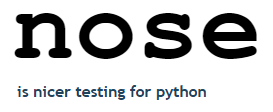
\includegraphics[width=0.25\columnwidth]{nose.png} 
    \caption{nose}
    \label{logo:company}
\end{figure}    
\subsection*{pycodestyle (pep8) - pylint}
Analisi statica del codice per Python. Rileva, a ogni salvataggio, errori di formattazione e di stile nel codice. Questi strumenti mi hanno permesso di mantenere un codice pulito, rispetto allo standard \glsfirstoccur{PEP8}. 
\begin{figure}[H]
    \centering
    
\includegraphics[width=0.3\columnwidth]{pylint.png} 
    \caption{Agile}
    \label{logo:company}
\end{figure}

\subsection*{NLTK}
Framework di python per la creazione di sinonimi, attraverso dizionari italiani e inglese.
\begin{figure}[H]
    \centering
    
\includegraphics[width=0.2\columnwidth]{nltk.png} 
    \caption{NLTK}
    \label{logo:company}
\end{figure}

\subsection*{TreeTagger}
Applicazione per l'estrazione dei lemma dalle parole. Viene adattato in Python attraverso \textit{TreeTaggerWrapper}.

\subsection*{Engagent}
Piattaforma sviluppata da {\company} formata dalla chatbot, il motre semantico e servizi di supporto. \'E servita per eseguire i test di sistema e accettazione, in quanto target dei file di configurazione generati dalla applicazione sviluppata durante lo stage.

\subsection{pip - PyPI}
\textbf{pip} è un sistema di gestione di pacchetti di Python. Semplifica il processo di installazione, aggiornamento e rimozione di pacchetti Python, attraverso semplici comandi. Permette il tracciamento delle dipendenze utilizzate dal programma. Tramite \textit{pip-env}, è possibile utilizzare un ambiente virtuale per garantire la portabilità dell'applicazione.\\
\textit{pip} mi ha permesso di eseguire eficientemente i seguenti task:
\begin{itemize}
    \item individuazione, installazione e tracciamento dei pacchetti di Python;
    \item installazione dell'applicazione nel server aziendale remoto, contenente il sistema operativo Linux.
\end{itemize}

%**************************************************************
\section{Progettazione}
%TODO AGGIUNGERE PROGETTAZIONE PIU' SPECIFICA DI OGNI CICLO DI SVILUPPO (MODEL, PRIMO BUILDER, STEMMER ECC.)
\label{sec:progettazione}
Durante lo stage, la progettazione è stata inserita all'interno del Manuale dello sviluppatore (documento in possesso di \company). Di seguito riporto tale progettazione, tralasciando però alcuni dettagli di implementazione, come richiesto dal tutor aziendale.

\subsection{Struttura dell'applicazione}
\begin{figure}[H]
    \centering
    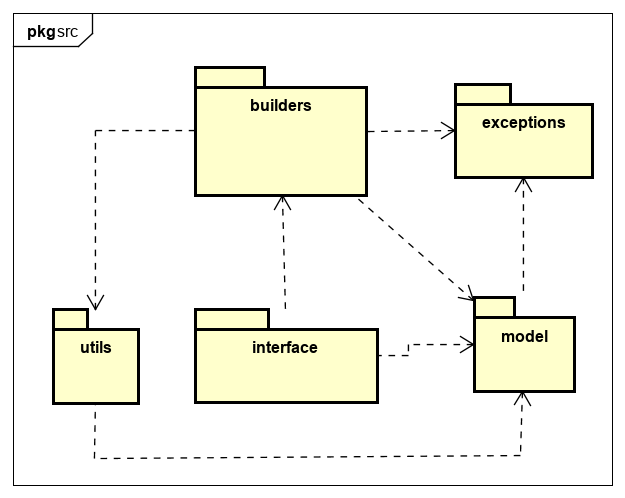
\includegraphics[width=0.7\columnwidth]{uml/packages.png} 
    \caption{Diagramma dei package}
    \label{logo:company}
\end{figure}

\subsubsection{model} %**************************
Le classi in \glsfirstoccur{model} rappresentano una configurazione \textit{NLP}.

\begin{namespacedesc}
    \classdesc{NLP}{Classe principale di \textit{model}, rappresenta una configurazione NLP. Le altre classi sono dei componenti di questa. Il metodo principale è "to\_string", che trasforma un oggetto NLP nella configurazione per \textit{Engagent}.}
    \classdesc{Rule}{Rappresenta una singola regola. Comprende il commento della regola, i \textit{match}, le domande e le risposte.}
    \classdesc{Synset}{Rappresenta un singolo synset. \'E composta da un titolo, alcuni valori di configurazione e i sinonimi.}
    \classdesc{Match}{Rappresenta un singolo match di una regola. \'E composta da un insieme di categorie, la priorità del match e un titolo.}
\end{namespacedesc}
\begin{figure}[H]
    \centering
    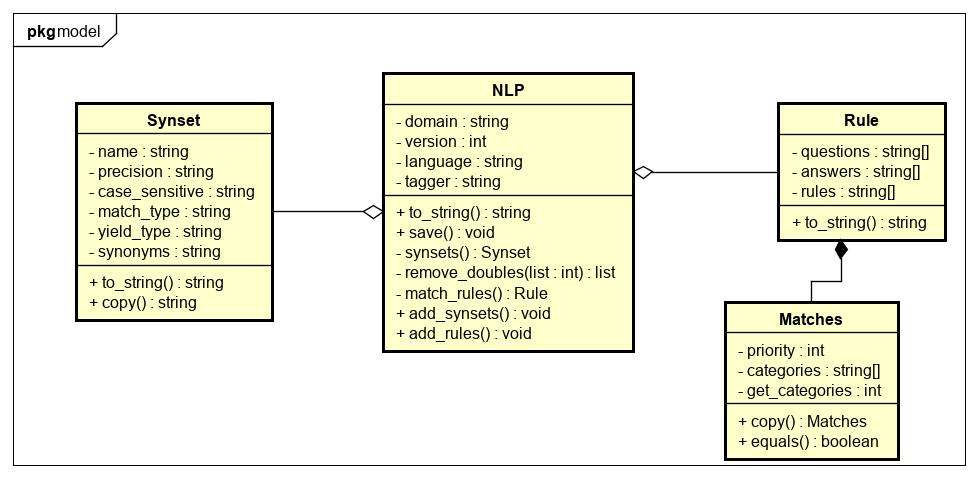
\includegraphics[width=0.7\columnwidth]{uml/model.png} 
    \caption{model}
    \label{logo:company}
\end{figure}

\subsubsection{builders} %**************************
Le classi in \textit{builders} permettono di creare un oggetto NLP, senza preoccuparsi della logica di implementazione. Attraverso il design pattern \textit{abstract method}, è possibile derivare la classe NLPBuilder, per creare builders che lavorano con formati diversi da JSON e XLSX.

\begin{namespacedesc}
    \classdesc{NLPBuilder}{Classe astratta per la creazione di un NLP. Contiene la logica principale di creazione delle configurazioni. Le classi che estendono questa classe devono solamente implementare i metodi astratti per standardizzare l'input (come definito nei commenti al codice e nel manuale dello sviluppatore).}
    \classdesc{NLPBuilderXLSX}{Classe che estende NLPBuilder. Standardizza l'input nel formato xlsx (excel).}
    \classdesc{NLPBuilderJSON}{Classe che estende NLPBuilder. Standardizza l'input nel formato json.}
\end{namespacedesc}
Nel diagramma è stato inserito anche il package \textit{model} per specificare cosa crea ogni builder.
\begin{figure}[H]
    \centering
    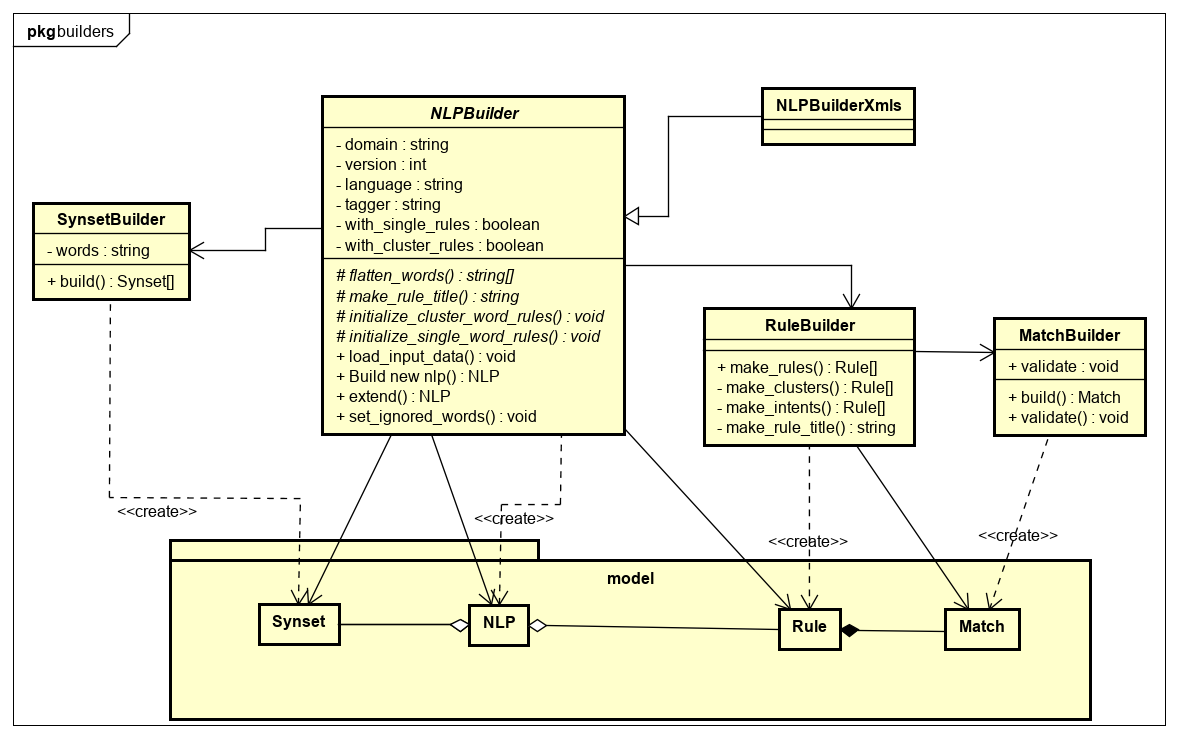
\includegraphics[width=0.7\columnwidth]{uml/build.png} 
    \caption{model}
    \label{logo:company}
\end{figure}
\subsubsection{utils} %**************************
Contiene moduli e classi di utilità.

\begin{namespacedesc}
    \classdesc{SynsetGenerator}{Questa classe contiene la logica di \textit{business} del programma, ovvero quella che esegue la vera trasformazione dell'input in \textit{synset} e regole (a differenza del model, che si limita a tradurre tali risultati in qualcosa di compatibile con Engagent). Questa classe utilizza la libreria NLTK e TreeTagger.}
    \classdesc{Utils}{Modulo che contiene funzioni di utilità, utilizzate da più classi non dipendenti tra di loro.}
    \classdesc{NLPStemmer}{Esegue lo stemming su un oggetto di tipo NLP.}
\end{namespacedesc}
\begin{figure}[H]
    \centering
    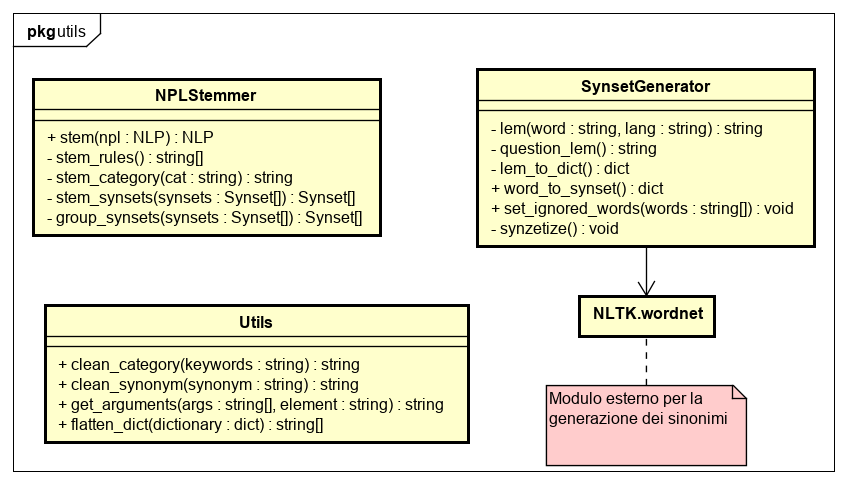
\includegraphics[width=0.7\columnwidth]{uml/utils.png} 
    \caption{model}
    \label{logo:company}
\end{figure}
\subsubsection{interface} %**************************
Interfaccia dell'applicazione per l'utente. Permette l'interazione programmatica e a linea di comando.

\begin{namespacedesc}
    \classdesc{api}{Permette l'interazione programmatica con l'applicazione.}
    \classdesc{cli}{Permette l'interazione a linea di comando con l'applicazione.}
\end{namespacedesc}

\subsubsection{exceptions} %**************************
Eccezioni personalizzate per l'applicazione.

\begin{namespacedesc}
    \classdesc{EmptyCategoryException}{Durante l'esecuzione del programma, è stata trovata una categoria vuota.}
    \classdesc{EmptySynonymException}{Durante l'esecuzione del programma, è stato trovato un sinonimo vuoto.}
\end{namespacedesc}

%**************************************************************
\section{Design Pattern utilizzati}
L'applicazione è stata sviluppata utilizzando i seguenti design pattern:
\begin{itemize}
    \item \textbf{Builder Pattern:} la creazione di un oggetto NLP può essere complicata, perché composta da almeno quattro componenti diverse. Il builder pattern permette di semplificare questo compito, rendendo di conseguenza le classi in \textit{model} meno complesse;
    \item \textbf{Abstract Pattern:} permette di aggiungere nuovi formati in input all'applicazione senza dover riscrivere l'intera logica di creazione dell'NLP.
\end{itemize}  

%**************************************************************
\section{Codifica}
\subsection{Task della codifica}
La codifica è stata intervallata con periodi di progettazione e analisi delle nuove richieste del tutor.
Per ogni nuova componente da sviluppare, ho seguito questi passaggi:
\begin{itemize}
    \item analisi e progettazione di dettaglio del problema;
    \item ricerca di soluzioni già esistenti per questo problema;
    \item codifica di quanto progettato e sviluppo di test di unità specifici;
    \item esecuzione di tutti i test di unità e risoluzione di eventuali \textit{bug};
    \item verifica da parte del tutor aziendale;
    \item risoluzione di eventuali errori logici.
\end{itemize}

\subsection{Stile del codice}
Per facilitare il lavoro di chi dovrà manutenere il progetto, ho seguito le linee guida definite in \textit{PEP8}\footnote{\url{https://www.python.org/dev/peps/pep-0008/}} per la stesura del codice:
\begin{itemize}
    \item i metodi più significativi sono documentati con il seguente commento:
    \begin{lstlisting}
        """[Descrizione]

        Arguments:
            arg1 {[tipo]} -- [descrizione]
        Returns:
            [tipo] -- [descrizione]
        Raises:
            [exception] -- [descrizione]
        """
    \end{lstlisting}
    \item le variabili private iniziano con un doppio underscore '\_\_';
    \item le variabili protette iniziano con un singolo underscore '\_';
    \item le variabili sono scritte interamente in minuscolo, variabili composte da più parole sono seprarate da underscore (esempio: get\_name)
\end{itemize}

\subsection{Codice significativo}

Di seguito, ho riportato degli esempi di codice significativo.
\subsubsection*{Implementazione di abstract method}
L'\textit{abstract method pattern} è stato utilizzato nella classe NLPBuilder. Il ruolo dei metodi astratti è lasciare alle classi derivate il compito di implementare la logica di trasformazione dell'input in un formato standard. Questo è il minimo neccessario richiesto per implementare un nuovo builder (per un nuovo formato di input).
\newline\newline
L'implmenetazione del metodo \textit{load\_input\_data} richiede la creazione di una variabile contenente il contenuto del file di input. Questa variabile verrà utilizzata solamente dalle implementazioni degli altri metodi astratti, quindi non è predefinita.
\begin{lstlisting}[language=python]
    @abstractmethod
    def load_input_data(self, path: str):
        """load the configuration from a file

        Arguments:
            path {str} -- relative path to the file
        """
        pass
\end{lstlisting}
Il metodo \textit{\_flatten\_words} estrae le categorie dall'input definito in \textit{load\_input\_data}. Gli altri metodi astratti definiti in NLPBuilder seguono una logica simile.
\begin{lstlisting}
    @abstractmethod
    def _flatten_words(self) -> list:
        """Flatten a list of categories in the input variable defined by load_input_data.

        Returns:
            words {list} -- of categories. E.g. ['dog','cat',plain','airplain']
        """
        pass
\end{lstlisting}